\documentclass[border=5pt]{standalone}
\usepackage{tikz}
\usepackage{amsmath,amssymb,bm}
\usetikzlibrary{arrows.meta, patterns}

\begin{document}
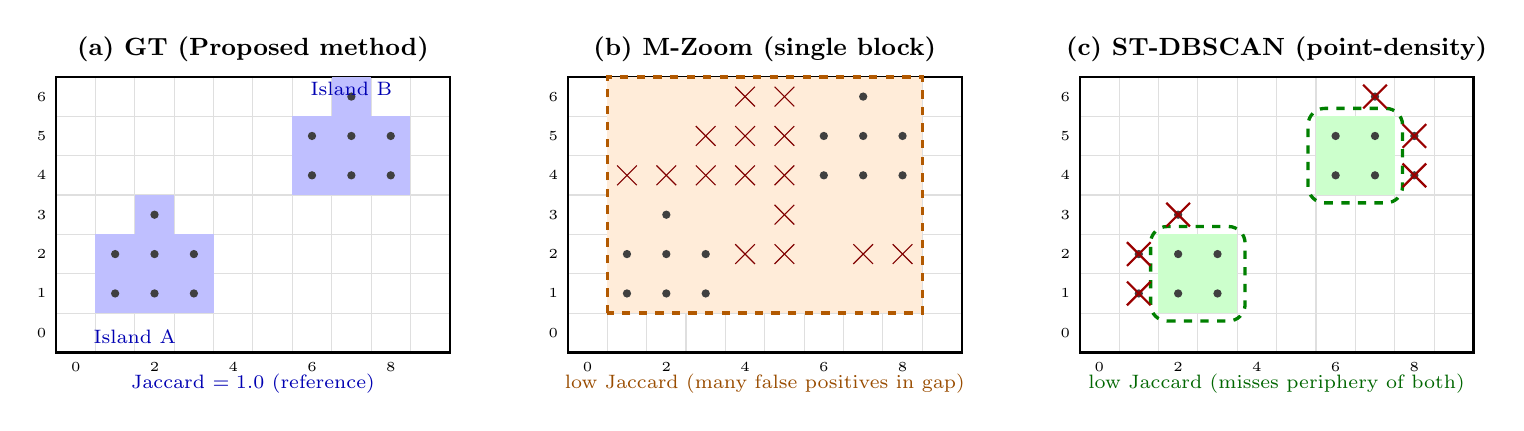
\begin{tikzpicture}[scale=0.50, every node/.style={font=\small}]

% ============================================================
% Helper macro for a small grid
% ============================================================
\newcommand{\drawgrid}[1]{
  \begin{scope}[shift={#1}]
    \draw[gray!25, thin] (0,0) grid[step=1] (10,7);
    \draw[thick] (0,0) rectangle (10,7);
    \foreach \x in {0,2,...,8}
      \node[below, font=\tiny] at (\x+0.5, 0) {\x};
    \foreach \y in {0,...,6}
      \node[left, font=\tiny] at (0, \y+0.5) {\y};
  \end{scope}
}

% ============================================================
% GT: Two islands
%   Island A (lower-left): t in [1,4], s in [1,3]
%   Island B (upper-right): t in [6,9], s in [4,6]
% ============================================================

% ============================================================
% (a) Ground Truth  —  proposed method detects both islands
% ============================================================
\drawgrid{(0,0)}
\node[font=\bfseries\small] at (5, 7.7)
  {(a) GT (Proposed method)};

\begin{scope}
% Island A: lower-left
\foreach \t/\s in {
  1/1, 2/1, 3/1,
  1/2, 2/2, 3/2,
  2/3
}{
  \fill[blue!25] (\t, \s) rectangle ++(1,1);
  \fill[black!75] (\t+0.5, \s+0.5) circle (3pt);
}

% Island B: upper-right
\foreach \t/\s in {
  6/4, 7/4, 8/4,
  6/5, 7/5, 8/5,
  7/6
}{
  \fill[blue!25] (\t, \s) rectangle ++(1,1);
  \fill[black!75] (\t+0.5, \s+0.5) circle (3pt);
}

% Labels for islands
\node[font=\scriptsize, blue!70!black] at (2, 0.4) {Island A};
\node[font=\scriptsize, blue!70!black] at (7.5, 6.7) {Island B};
\end{scope}

% Jaccard label
\node[font=\scriptsize, blue!70!black] at (5, -0.8)
  {Jaccard $= 1.0$ (reference)};

% ============================================================
% (b) M-Zoom  —  Cartesian product block (bounding box)
% ============================================================
\drawgrid{(13,0)}
\node[font=\bfseries\small] at (18, 7.7)
  {(b) M-Zoom (single block)};

\begin{scope}[shift={(13,0)}]
% M-Zoom outputs bounding-box: t in [1,9] x s in [1,6]
\fill[orange!15] (1,1) rectangle (9,7);
\draw[orange!70!black, very thick, dashed] (1,1) rectangle (9,7);

% GT dots (Island A)
\foreach \t/\s in {
  1/1, 2/1, 3/1,
  1/2, 2/2, 3/2,
  2/3
}{
  \fill[black!75] (\t+0.5, \s+0.5) circle (3pt);
}

% GT dots (Island B)
\foreach \t/\s in {
  6/4, 7/4, 8/4,
  6/5, 7/5, 8/5,
  7/6
}{
  \fill[black!75] (\t+0.5, \s+0.5) circle (3pt);
}

% False positive X marks (cells in bounding box but not GT)
% Representative FP cells in the gap between islands
\foreach \t/\s in {
  4/2, 5/2, 5/3,
  4/4, 5/4, 3/4,
  4/5, 5/5, 3/5,
  4/6, 5/6,
  1/4, 2/4, 7/2, 8/2
}{
  \draw[red!50!black, thin] (\t+0.25, \s+0.25) -- (\t+0.75, \s+0.75);
  \draw[red!50!black, thin] (\t+0.75, \s+0.25) -- (\t+0.25, \s+0.75);
}

% Label
\node[font=\scriptsize, orange!60!black] at (5, -0.8)
  {low Jaccard (many false positives in gap)};
\end{scope}

% ============================================================
% (c) ST-DBSCAN  —  point-density clusters (imprecise boundaries)
% ============================================================
\drawgrid{(26,0)}
\node[font=\bfseries\small] at (31, 7.7)
  {(c) ST-DBSCAN (point-density)};

\begin{scope}[shift={(26,0)}]
% ST-DBSCAN finds both clusters but with imprecise boundaries:
%   - misses peripheral cells (low local density at edges)
%   - may include extra cells near dense cores

% Detected cluster A (core only, misses periphery)
\foreach \t/\s in {
  2/1, 3/1,
  2/2, 3/2
}{
  \fill[green!20] (\t, \s) rectangle ++(1,1);
}

% Cluster A outline (rounded = point-neighborhood shape)
\draw[green!50!black, very thick, dashed, rounded corners=6pt]
  (1.8, 0.8) -- (4.2, 0.8) -- (4.2, 3.2)
  -- (1.8, 3.2) -- cycle;

% Detected cluster B (core only, misses periphery)
\foreach \t/\s in {
  6/4, 7/4,
  6/5, 7/5
}{
  \fill[green!20] (\t, \s) rectangle ++(1,1);
}

% Cluster B outline
\draw[green!50!black, very thick, dashed, rounded corners=6pt]
  (5.8, 3.8) -- (8.2, 3.8) -- (8.2, 6.2)
  -- (5.8, 6.2) -- cycle;

% All GT dots
\foreach \t/\s in {
  1/1, 2/1, 3/1,
  1/2, 2/2, 3/2,
  2/3
}{
  \fill[black!75] (\t+0.5, \s+0.5) circle (3pt);
}
\foreach \t/\s in {
  6/4, 7/4, 8/4,
  6/5, 7/5, 8/5,
  7/6
}{
  \fill[black!75] (\t+0.5, \s+0.5) circle (3pt);
}

% Missed cells (GT but not in detected cluster)
\foreach \t/\s in {
  1/1, 1/2, 2/3,
  8/4, 8/5, 7/6
}{
  \draw[red!60!black, thick] (\t+0.2, \s+0.2) -- (\t+0.8, \s+0.8);
  \draw[red!60!black, thick] (\t+0.8, \s+0.2) -- (\t+0.2, \s+0.8);
}

% Label
\node[font=\scriptsize, green!40!black] at (5, -0.8)
  {low Jaccard (misses periphery of both)};
\end{scope}

\end{tikzpicture}
\end{document}
